\section{Introduction}

IoT devices have become an essential part of our daily lives in commercial, industrial, and infrastructure systems. These devices offer benefits to consumers by interacting with the physical environment through sensors and actuators, which allows device automation thereby improving efficiency. Unfortunately, the proliferation of IoT devices has led to an increase in the number of remotely exploitable vulnerabilities leading to new attack vectors that could have disastrous financial and physical implications. In 2015, security researchers demonstrated a vulnerability on the Jeep vehicle which allowed remote control of the automotive system over the Internet \cite{jeep_vulnerabilty}. In 2016, researchers discovered a vulnerability that allows Internet connected smart thermostats to be subject to remote ransomware attacks in which an attacker gains sole control of the thermostat until a fee is paid \cite{smart_thermostat}. These are a few examples of some of the potential malicious vulnerabilities that could have devastating, long-lasting impact on an IoT system. \par Intrusion detection \cite{Lazarevic2005} is the process of discovering malicious exploits in a system. One way of detecting an intrusion is by the use of anomaly detection techniques. An anomaly, also referred to as an outlier, is data that deviates from the normal system behavior. Anomalies could be indicative of a system fault or that a system has been compromised by a malicious event. Due to the sensitive nature of safety critical systems, detecting malicious attacks is of utmost importance.

 
%\par Sensors and actuators are important components of an IoT device. Sensors detects environmental signals which are relayed as electric or optical output. An actuator on the other hand, performs task specified by a control signal (e.g sensor's signal or manual input). From pacemakers to motor vehicles, IoT devices generate an unprecedented amount  of sensor data, it is important to track the information flow of sensor based events in order to uncover anomalous relationships that exists between sensor based events in an IoT device. In this paper, we motivate the need for IoT device anomaly detection.



% \par Unlike most host-based intrusion detection system which utilize system call frequencies to determine anomalous system events, our approach detects anomalies by leveraging the information flow of sensor events as represented in a provenance graph. Provenance graph captures a comprehensive history of transformations that occurs on a data object during its lifecycle. It offers a way of representing relationships that exist between multiple data objects. This, in turn, can be used to detect system faults or anomalous system events such as malicious intrusions. 
 
 
 \par We propose an approach to identifying anomalous sensor events using provenance graphs. This approach involves the use of a similarity metric to compare observed provenance graphs with provenance graphs derived from an application's normal execution. The result is an anomaly score which is  compared with a previously set threshold to classify an observed provenance graph as either anomalous or benign. We evaluate the effectiveness of our approach with a sample IoT application that simulates a climate control system.




%\par In summary, our technical contributions are outlined in detail as follows:
%
%
%%Anomaly detection has applications in domains such as intrusion detection, fraud detection, medical health devices, sensor fault detection, and web spam.
%
%
%
%%We also propose a hybrid classification algorithm based on $k$- Nearest Neighbors ($k$-NN), and $k$ means clustering. Anomalous events are detected based on their proximity to known normal provenance graph. Our technical contributions are outlined in detail as follows:
%
%\begin{itemize}[]
%
%\item We introduce an anomaly detection algorithm for detecting malicious intrusions in an IoT device using provenance graphs. 
%
%%\item We take a hybrid approach to anomaly detection by combining clustering, classification, and density-based techniques. In the training phase, the unlabeled data set is clustered into two groups (where $k \lesssim 2$). The density of each cluster is observed using the Local Outlier Factor (LOF) to determine which cluster is considered the normal or an anomaly. In the test phase,  $k$ nearest neighbor algorithm is used to classify incoming data instances as normal or anomaly.
%
%%\item We propose two anomaly detection techniques for IoT devices using provenance graphs. The first algorithm is based on the similarity between provenance graphs in the learning and detection phases which is achieved by using a similarity metric. The second algorithm is a hybrid approach which uses clustering algorithm, DBSCAN, and $k$-nearest neighbor algorithm.
%
%
%
%\item We evaluate the effectiveness of our approach to anomaly detection with a dataset from an IoT application by comparing the false positive, false negative and true positive rate of our proposed approach. Detailed results are presented in sections V. 
%
%\end{itemize}

%The remaining portion of this paper is organized as follows. In section 2, we discuss background information on anomaly detection and provenance graphs. In section 3, we describe our threat model and assumptions, In section 4, we discuss details of our graph based anomaly detection algorithm. In section 5, we describes our experimental design and evaluation. In section 6 we describe related work on intrusion detection and graph based anomaly detection. Finally, in section 7, we summarize and conclude our findings.



%Graph based anomaly detection has been explored in various research.Most of the prior work focuses on static graphs using community outliers, and finding similarities from frequent substructures. 

%There are two major approach to intrusion detection. Signature based Intrusion detection and anomaly based detection.











%\section{Problem Statement}
%
%Given a set of provenance graphs, P = $\{p_1, p_2,...p_n\}$ containing provenance data from both the learning and detection phase, we want detect anomalies that might exist in P.  This involves converting elements in $P$ into a feature vector space. Anomalies are detected by comparing the similarity of graphs contained in $P$ using a similarity metric and also by using a hybrid approach as discussed in section IV


% Anomalies are detected using a hybrid approach which is a combination of clustering and classification algorithms discussed in section IV

\section{Graph Similarity Anomaly Detection}

%This section describes key concepts of Anomaly detection techniques, Provenance graphs, text-based query ranking and $k$-NN. 

\subsection{Provenance Graphs}
%An example of provenance can be seen with a college transcript. A transcript is the provenance of a college degree because it outlines all of the courses satisfied in order to attain a degree. In computing, d

Provenance denotes the origin of an object and all other activities that occurred on that object. Data provenance, also known as data lineage, can be defined as the history of all activities performed on a data object from its creation to its current state. Provenance ensures data trust \cite{Bertino2015}. It establishes causality between entities contained in a data object through information flow tracking thereby it allows for the verification of a data source. Provenance is represented by a directed acyclic graph (DAG) in which vertices represent data entities and the edges correspond to the interaction between them. 

%\begin{figure}[h!]
%\begin{center}
%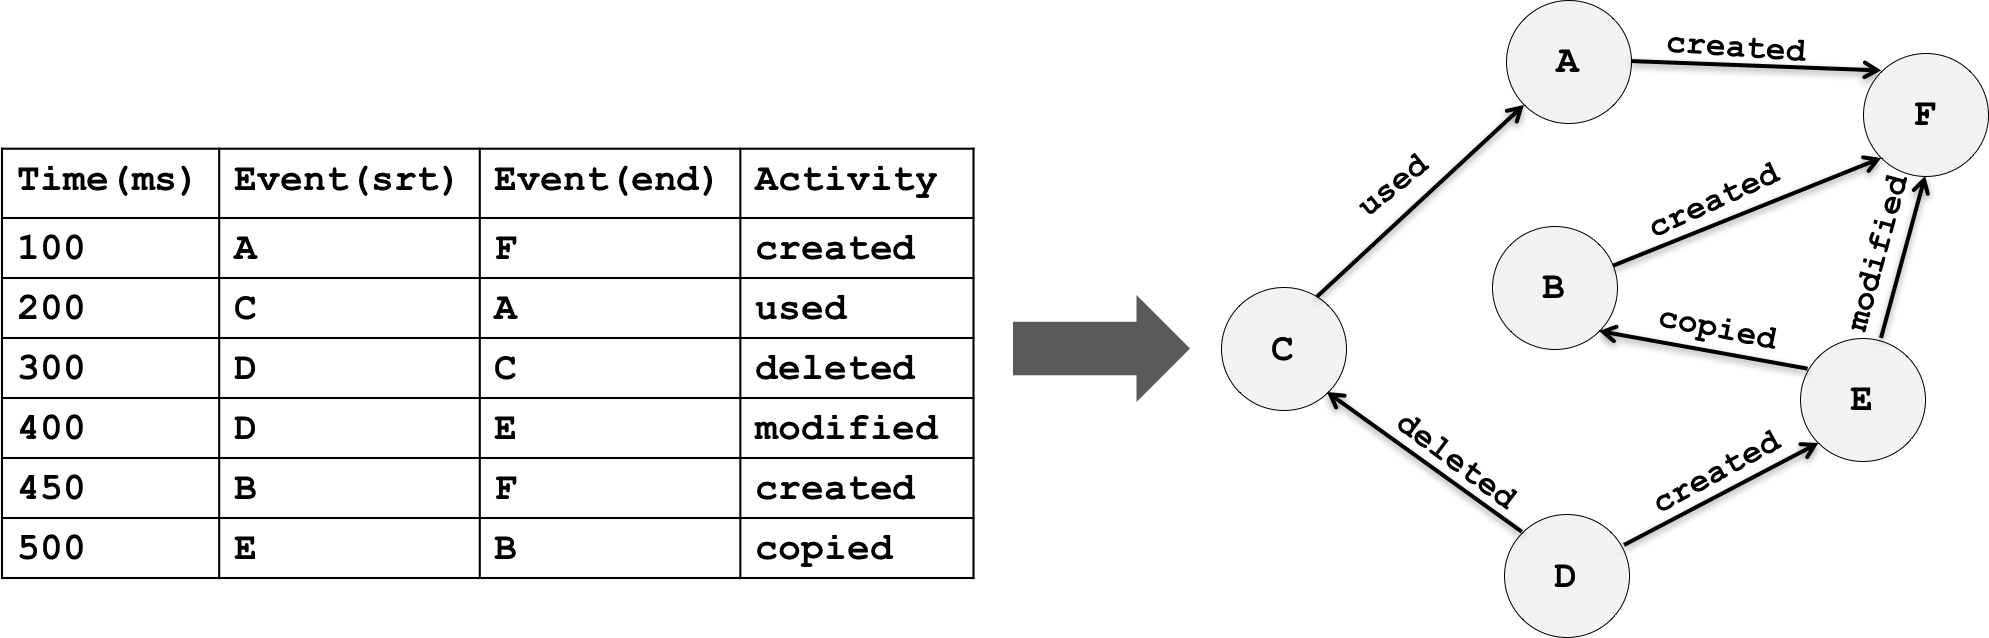
\includegraphics[height=1.4in, width=3.5in]{provenance_graph_2.png}
%\end{center}
%\caption{Provenance data transcribed to Provenance graph which depicts causal dependency between system events. The nodes represents events while the edges represents activities}
%\label{Provenance_graph}
%\end{figure}

\begin{figure}[h!]
\begin{center}
%\includegraphics[width=\columnwidth]{picture11.pdf}
%\includegraphics[width=\columnwidth]{picture12.pdf}
\includegraphics[width=\columnwidth]{picture1_edit.pdf}
\end{center}
\caption{Components of a provenance graph where nodes represent types (agent, activity, and entity) and edges represent relationships between types}
\label{Provenance_Sensor}
\end{figure}


Most provenance collection frameworks developed to track provenance use system level event sequences in an operating system \cite{pasquier-socc2017,acsac,Muniswamy-Reddy}. For IoT devices, containing limited or no operating system functionality, it is essential to use a provenance collection framework that places less emphasis on an operating system and more emphasis on application level information flow tracking. For our provenance graph generation, we use PAIoT \cite{paiot}, a provenance collection framework which tracks the information flow of sensor-based events in an IoT device. In PAIoT, sensor data containing observation information is represented as a provenance graph. Sensor events are instrumented in the application source code. Each sensor data generated is defined as a tuple $(t, e, a, s_1, r_1)$ where $t$ represents the time a sensor reading was generated, $e$ represents the sensor data, $a$ represents activity performed on sensor data, $ s_1$ represents a sensor identifier, and $r_1$ represents the device information. Tuple information is constructed as a provenance graph and stored in a graph database (Neo4j) where further processing and query analytics can be performed on provenance data.




%\par We formally define a provenance graph as follows: 


%\subsubsection{Provenance-Sensor Model}
%
%Trace data is mapped into a provenance graph representation by using the provenance-sensor model as defined in \cite{}. Provenance-sensor model denotes the information flow of sensor events leading to a decision point using provenance based ontology. Provenance-Sensor model consists of three major component: Agents, activity, and entities. We outline the components of the provenance-sensor model as follows:  

%A sensor trace is represented as a tuple $(t, e, a, s_1, r_1)$ where t is a timestamp, $e$ denotes an event, $a$ denotes an activity, $s_1$ denotes a sensor identifier and $r_1$ denotes a device identifier. There are a total of 7 edge labels between nodes in a provenance graph. These edges denote derivation, attribution, association, and generation relations.



%% 
%An event is the data that was produced by an activity.
%
%two vertices are equal if they have the same type and the same value...go to say they are no two events that are equal, events are distinct.
%
%Enitites are outputs to activities. An agent is 
%
%Get to the point of stating that a provenance graph is a set of vertices and edges and the vertices are of the three types, agent, entity, and activty
%
%
%
%Think about the vertices as abstract node, a field of nodes. A set of vertices that have the type agent, entity, and activity. The node value of a vertex includes a type. Depending on what type of node it is, it can have additional information in it.
%
%A directed graph is a set of vertices and edges, those vertices can be differentiated by their values. We make the distinction based the type and value in them. Where V is a set of vertices where each vertex has a type. The type can be one of three things, agent, entity, and activity and also a value. An agent value, is an identifier, entity's value is an event and an activity is an action. 






%\begin{figure}[h!]
%\begin{center}
%\includegraphics[height=2in, width=3.5in]{picture1.png}
%\end{center}
%\caption{Components of a provenance graph}
%\label{Provenance_Sensor}
%\end{figure}


%A provenance graph is a directed acyclic graph, $p = (V,E)$ where $V$ is a set of vertices $V =\{v_1,...,v_n\}$ such that $v_i = (label, type, value)$ and $E$ is a set of edges $E =\{e_1,..., e_n\}$ where $e_i = (v_s, v_d, label)$ and $v_s, v_d$ are source and destination vertices. Two vertices $v_x$, $v_y$ are similar (denoted $ v_x \sim v_y$) if $v_x.type = v_y.type$ and $v_x.value = v_y.value$. Two edges $e_x $ and $e_y$ are similar (denoted $e_x \sim e_y$) if $e_x.v_s \sim e_y.v_s$, $e_x.v_d \sim e_y.v_d$, and $e_x.label = e_y.label$. \textcolor{red}{ We define a union operator over a collection of edge set (denoted by $\cup$) as a set of non-similar edges contained in the edge set. For example, assume $E_i$ and $E_j$ are edge lists, $E_i \cup E_j = \{e_i: e_i \in E_i$ or $e_i \in E_j\}$}. Types may take on one of the following: Agent, Entity, and Activity.  An agent is an actor that is represented by an identifier (e.g., sensor or device name). An entity is an event, which represents data that is produced as a result of an activity. An activity is an action performed by an agent or entity (e.g., read, update, create, delete). $label$ takes on one of the following values: \textit{wasGeneratedBy}, \textit{used}, \textit{wasInformedBy}, \textit{wasDerivedFrom}, \textit{wasAttributedTo}, \textit{wasAssociatedWith}, \textit{actedOnBehalfOf}. 

% A decision point is a logical component of a provenance graph which denotes the evaluation of an action performed on an entity. 



A provenance graph is a directed acyclic graph, $p = (V,E)$ where $V$ is a set of vertices $V =\{v_1,...,v_n\}$ such that $v_i = (type, value)$ and $E$ is a set of edges $E =\{e_1,..., e_n\}$ where $e_i = (v_s, v_d, label)$ and $v_s, v_d$ are source and destination vertices. Two vertices $v_x$, $v_y$ are equal (denoted $ v_x = v_y$) if $v_x.type = v_y.type$ and $v_x.value = v_y.value$. Two edges $e_x $ and $e_y$ are equal (denoted $e_x = e_y$) if $e_x.v_s = e_y.v_s$, $e_x.v_d = e_y.v_d$, and $e_x.label = e_y.label$.  We use the union operator $\cup$ over edge sets in the usual way of the union of sets.}

Types may take on one of the following: Agent, Entity, and Activity.  An agent is an actor that is represented by an identifier (e.g., sensor or device name). An entity is an event, which represents data that is produced as a result of an activity. An activity is an action performed by an agent or entity (e.g., read, update, create, delete). $label$ takes on one of the following values: \textit{wasGeneratedBy}, \textit{used}, \textit{wasInformedBy}, \textit{wasDerivedFrom}, \textit{wasAttributedTo}, \textit{wasAssociatedWith}, \textit{actedOnBehalfOf}. 




\begin{figure*}
\begin{center}
%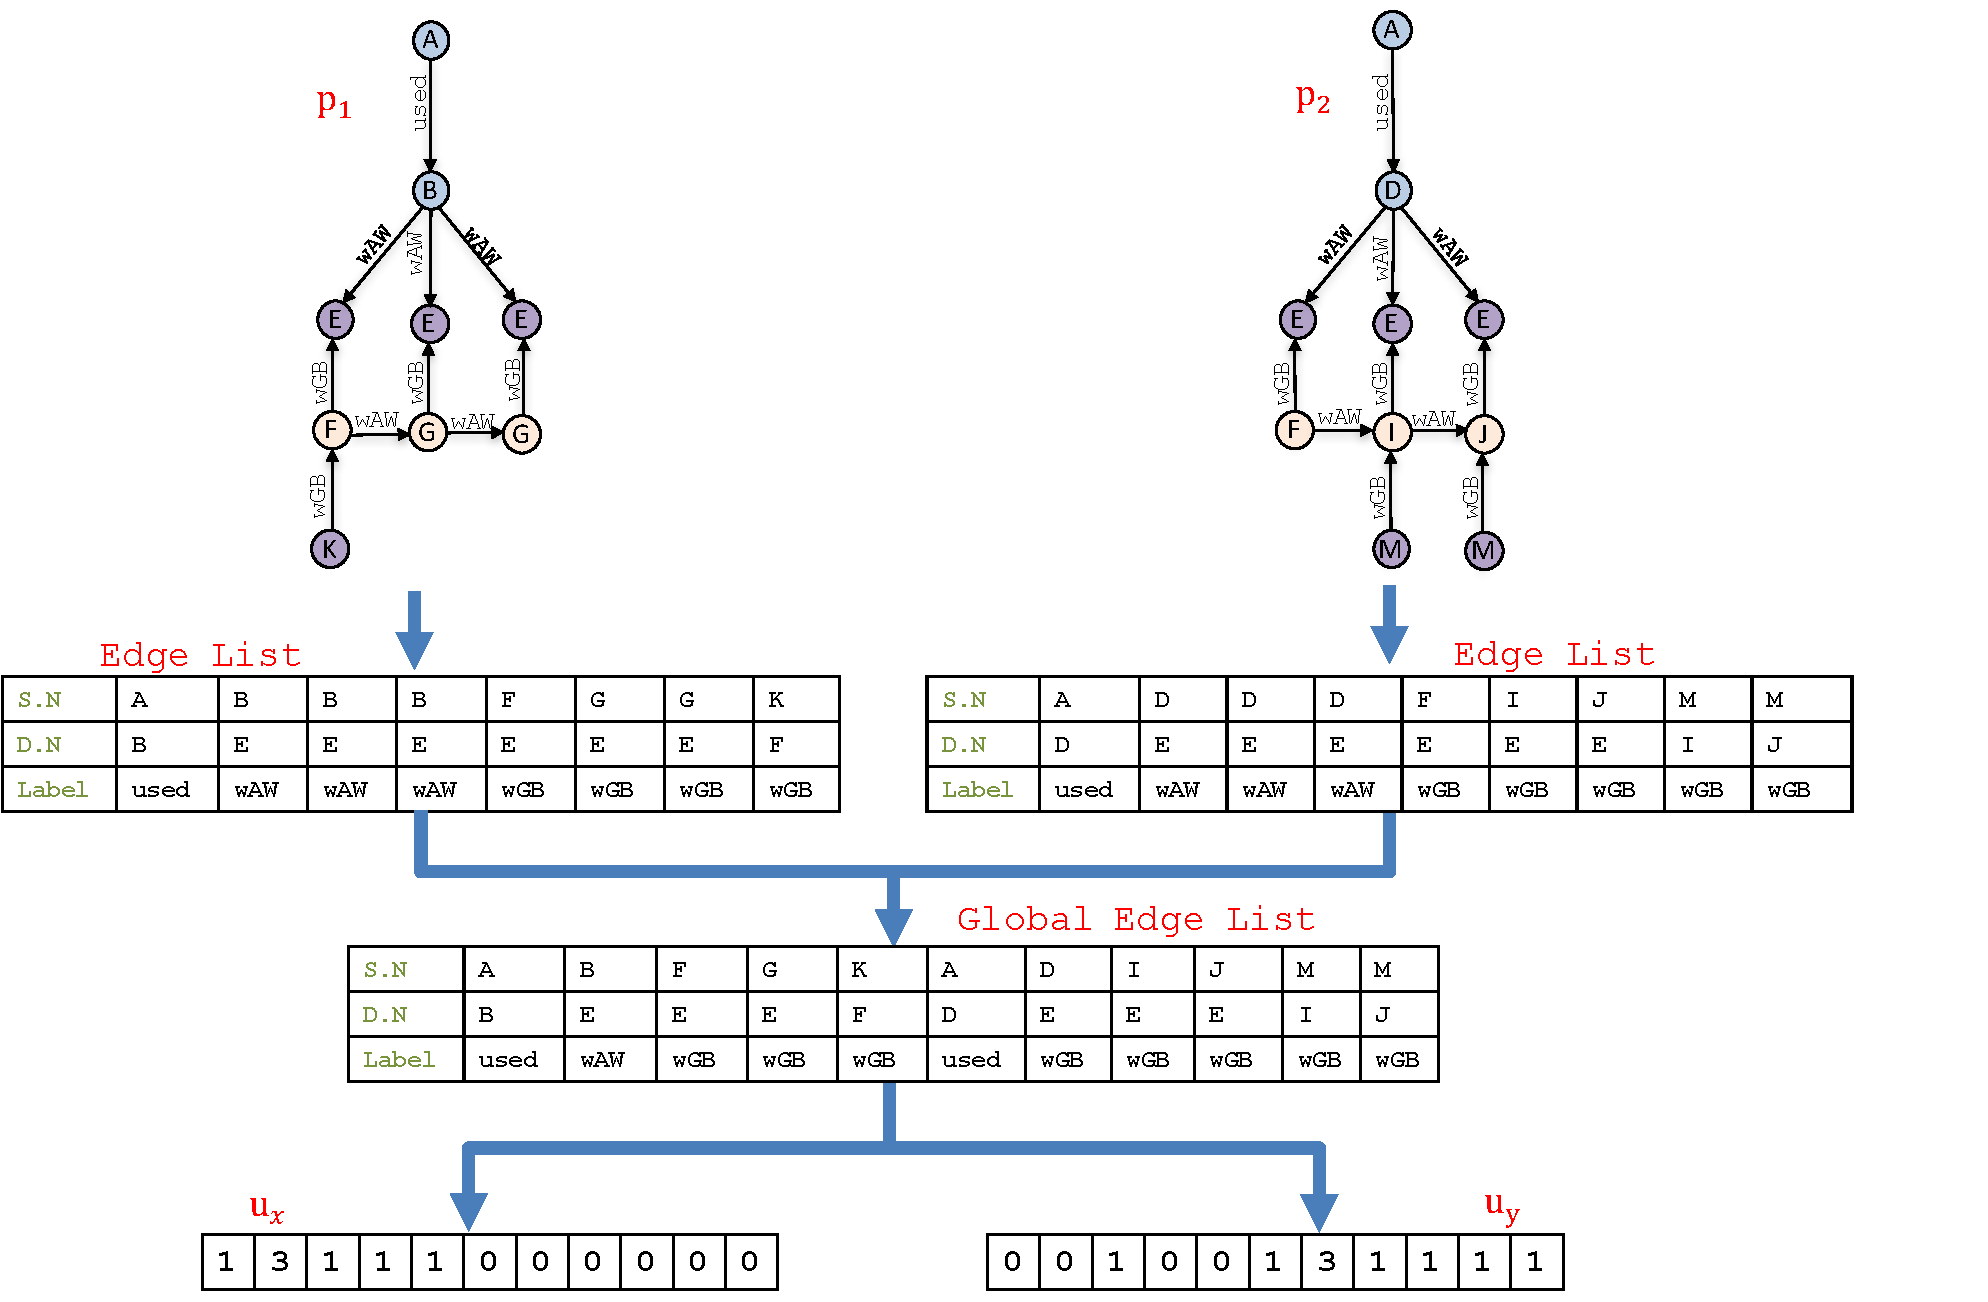
\includegraphics[width=\textwidth]{vector3.pdf}
%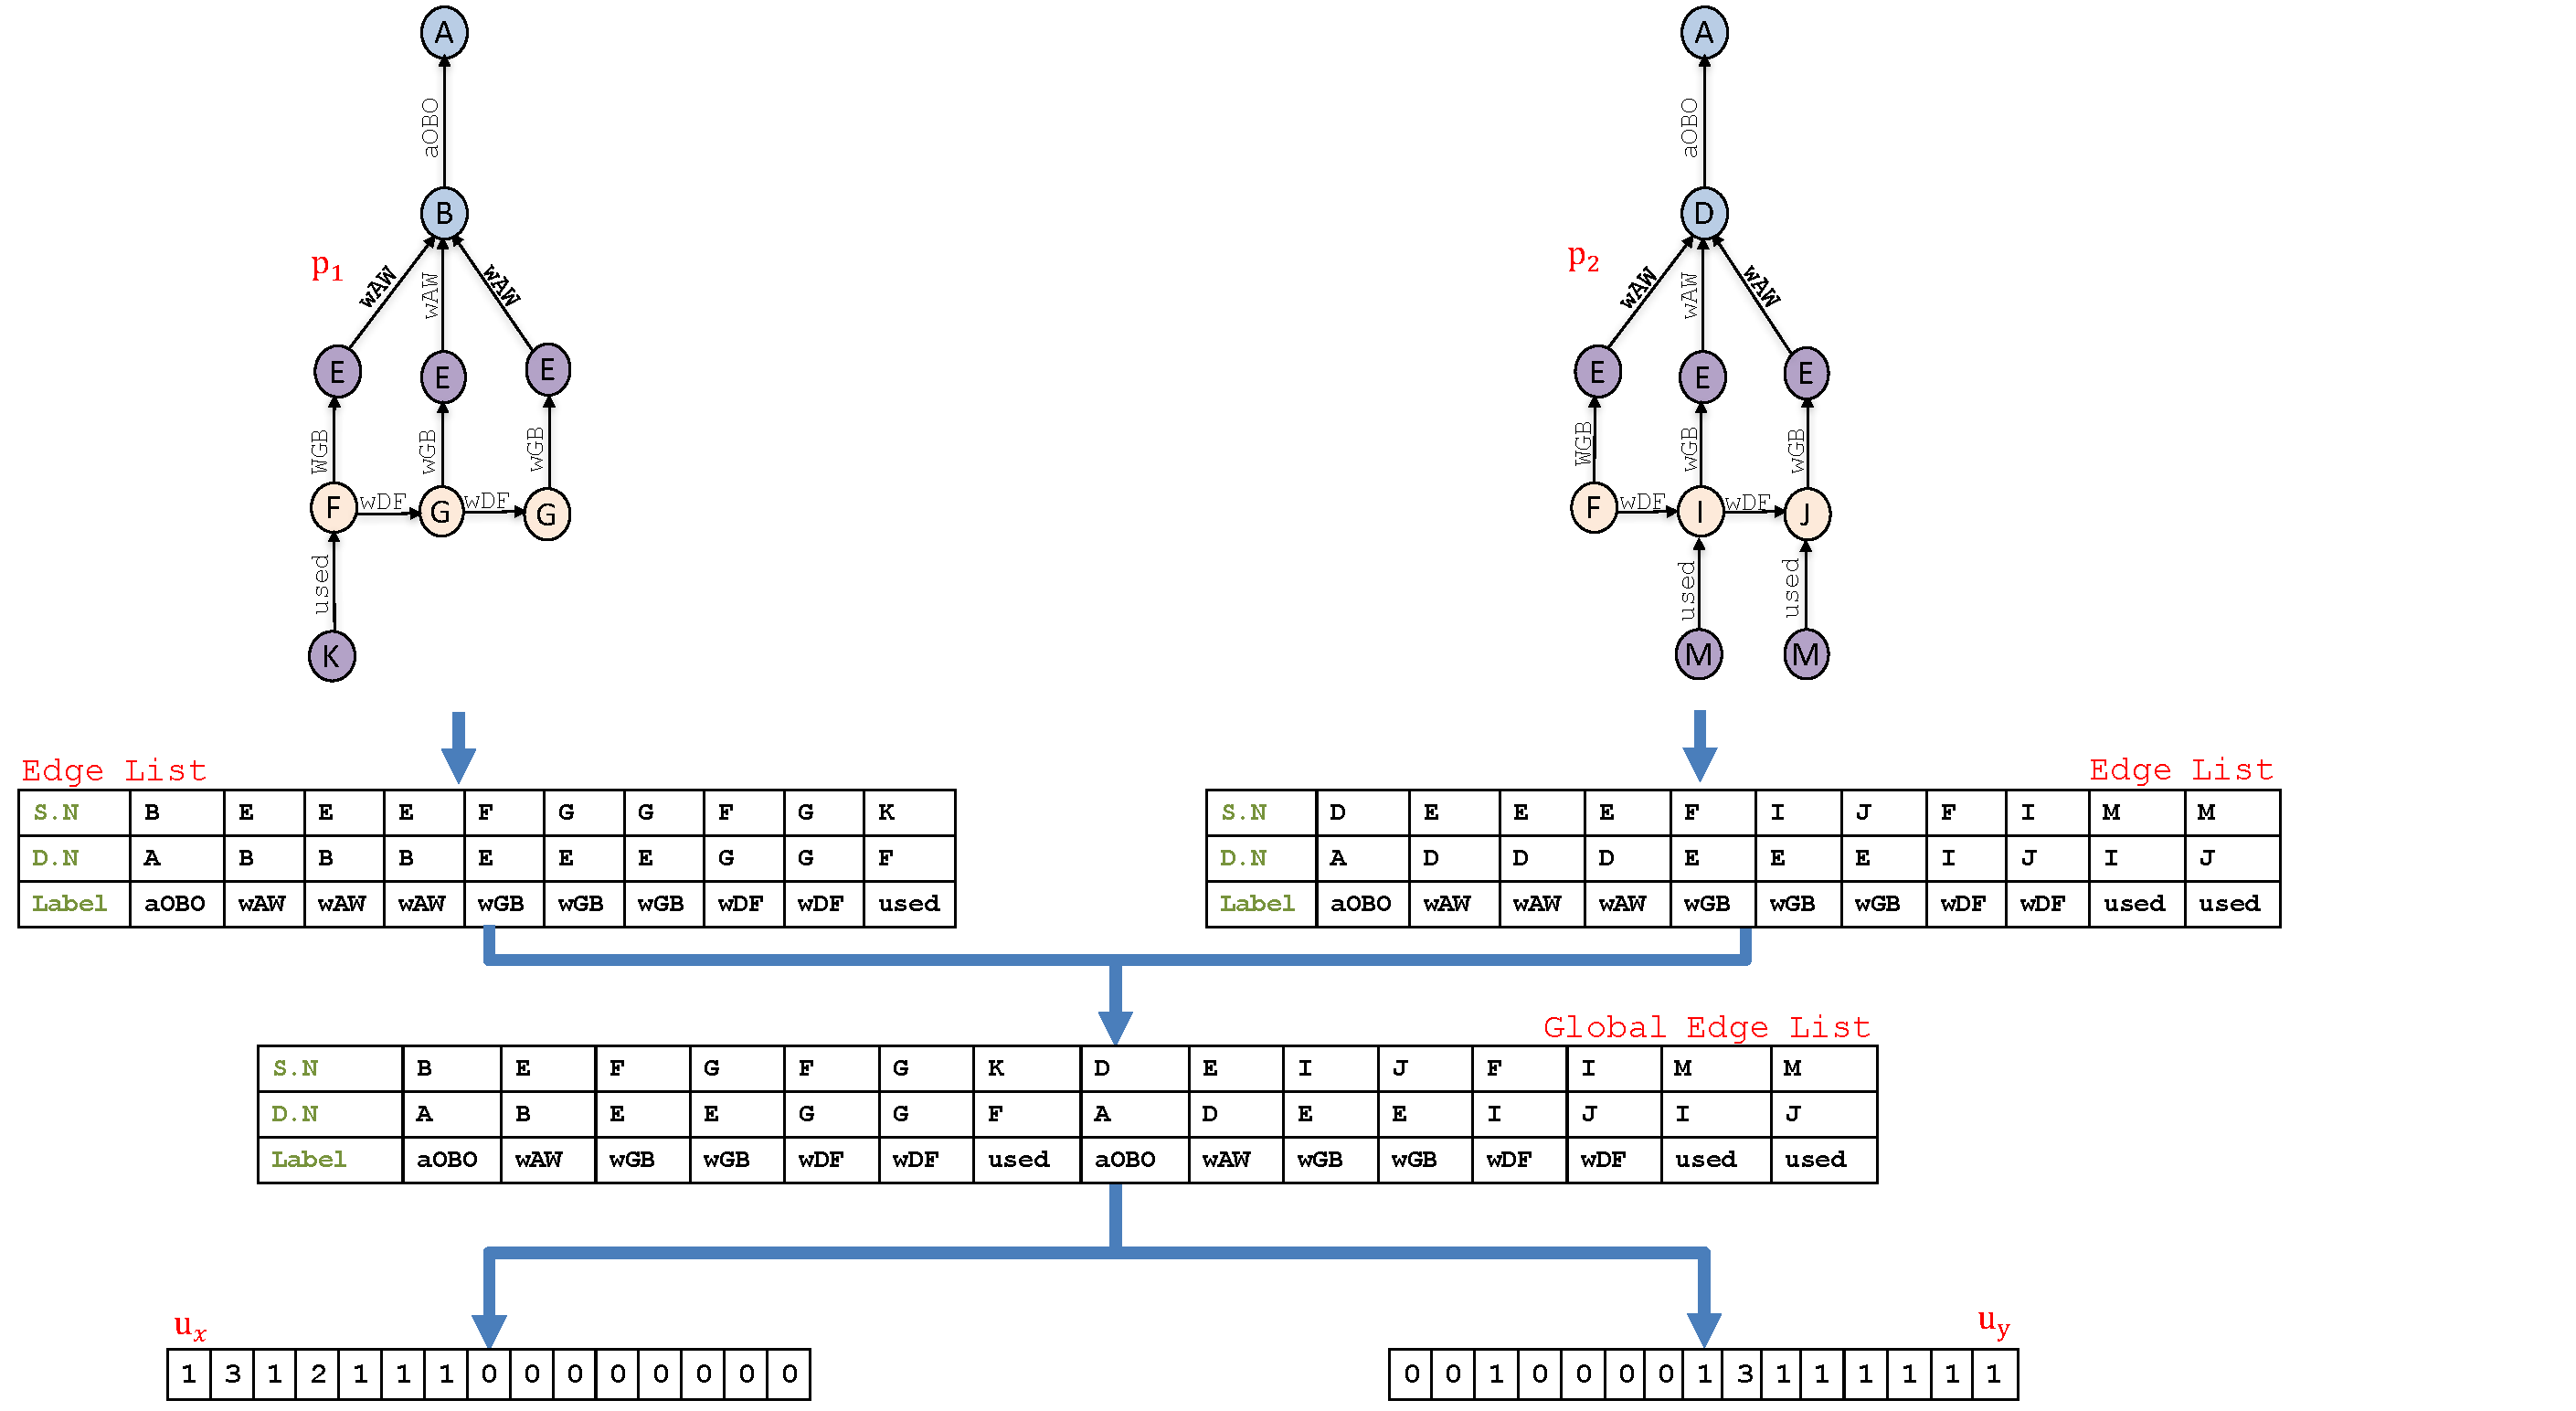
\includegraphics[width=\textwidth]{vector5.pdf}
\includegraphics[width=\textwidth]{picture13_edit_1.pdf}
\end{center}
\caption{Provenance graph conversion to vector space. $u_x, u_y$ represents vectors generated from both provenance graphs}
\label{prov_vector}
\end{figure*}



%In an IoT application, there exist recurrent design patterns which can be leveraged to understand data flow. This information, can be leveraged to define the expected provenance graph for each application. 



%\par There are two types of control systems: open and closed loop. In open loop control, the system's output is not affected by the conditions (i.e., there is no feedback loop). An example of an open loop control system is a microwave. The timer is manually set to determine when the microwave stops regardless of the condition of its content (e.g., if the food is properly heated). However, in closed loop control, the system's output is used as feedback to influence the input.  An example of a closed loop system is a thermostat in which the temperature serves as output which is also used as an input feedback to regulate the temperature based on a predefined set-point. 


 


%Causality and dependency are concepts used to denote relationship between system events. Provenance graphs in turn be used in digital forensics \cite{zhang_outlier_2010} to investigate the cause of a malicious attack and also in intrusion detection systems to further enhance the security of computing devices. For further reading on provenance models and provenance graphs, we refer the reader to \cite{}  


 





%\subsection{Provenance-system collection}
%
%\subsubsection{Observed Provenance}
%
%\subsubsection{Disclosed Provenance}



%\subsection{Provenance Characteristics}
%
%Since provenance denotes the who, where and why of data transformation, it is imperative that data disseminated in an IoT architecture satisfies the required conditions. The characteristics of data provenance are outlined in detail below.
%
%
%\begin{itemize}
%
%\item Who: This characteristic provides information on activities made to an entity. Knowing the ``who" characteristic is essential because it maps the identity of modification to a particular data object. An example of ``who" in an IoT use case is a sensor device identifier.
%
%\item Where: This characteristic denotes location information in which data transformation was made. This provenance characteristic could be optional since not every data modification contains location details.
%
%\item When: This characteristic denotes the time information at which data transformation occurred. This is an essential provenance characteristic. Being able to tell the time of a data transformation allows for tracing data irregularities.
%
%\item What: This characteristic denotes the transformation is applied on a data object. A use case for IoT can be seen in the various operations (create, read, update, and delete) that could be performed on a file object.
%
%\end{itemize}
%
%
%There are two ways of pruning Provenance data: Provenance can be pruned at collection before it is been committed to the disk  or after being recorded to disk. Policy defines rules and actions that should be taken if any of the rules applies.  Access control in this case is used as a tool for pruning provenance data stored on an IoT device. It can also be extended for traditional access control measures. Data pruning is an essential problem for automatic provenance collection. Observed provenance and disclosed provenance. Observed provenance involves automatic collection of system states and changes. One major drawback of this method is that all system events are provenanced including irrelevant system provenance which incurs more storage overhead. Described provenance on the other hand, allows a user to provide a workflow of how what provenance the system is intended to generate and an engine to execute the workflow described.

%\subsection{ Document retrieval using vector space model} 
%Vector space conversion is used in information retrieval technique for determining document similarity to a query. Given a corpus $D = \{ d_1,..., d_n\}$, a query, $q$,  find document(s) ${d_x,....d_y}$ which are similar to $q$ and rank them by order of importance. To achieve this, documents are converted into a vector space representation which allows document to be ranked based on some similarity metric.
%
%
%\subsubsection{term frequency-inverse document frequency:}
%
%term frequency - inverse document frequency (tf-idf) is a widely used weighting scheme for ranking documents in a corpus given a query. The algorithm reflects how important a word is to a document. The more common a word is in a document, the higher the weighting factor. Given a term $t$ in document $d$ the term frequency $tf(t,d)$ is the number of times $t$ occurs in $d$.  tf-idf is composed of two algorithms: term frequency $tf$ and inverse document frequency, $idf$ .  tf-idf is derived from the product of tf and idf.
%
%  \[ tf-idf(t,d, D) = tf(t,d) \times idf(t,D) \]
%
%\par There are a number of ways to calculating the term frequency of a document. The first approach counts the raw frequency of each word contained in the document. 
% 
%
%\[ tf(t,d) = freq(t,d) \]
%
% 
% Another approach is to use boolean weighting. If a word is contained in a document, a weight of 1 is assigned as the term frequency, otherwise, a weight of 0 is assigned.
% 
% Other ways of computing the term frequency involves the use of the normalized instances of the term frequency. (i.e by dividing the frequency of each words by the total number of words contained in the document or by using the log of the raw frequency)
%
%  \[ tf(t,d) = \dfrac{freq(t,d)}{N} \]
%  
%   
% \[ tf(t,d) =  \log{(freq(t,d))} \]
% 
% 
%One major drawback of using the term frequency is that all terms in a document are considered equal while retrieving a query.In a corpus, some documents might contain words that are commonly repeated in every other documents. This adversely influences the weighting factor of a term in a corpus. For instance, in a collection of documents, words like  "the" are widely used and might occur more frequently.  Inverse document frequency (idf) ensures that frequently occurring words in a list of documents are given a lower weight than less occurring words. The more frequent a term occurs in a corpus, the less the idf weight.
%
% idf is computed by taking the log of the total number of documents in a corpus , $N$ divided by the number of documents which contains the term $df_t$.
% 
% \[idf(t, D) =\log \dfrac{N}{df_t} \]
% 
%tf-idf weighting scheme provides a vector space representation of documents. To compare the similarity between two documents, we employ the use of  a similarity measure such as cosine similarity, Jaccard similarity or euclidean distance. This similarity measures calculates some form of distance between the two vectors. Cosine similarity has been shown to outperform the rest of the similarity measures in comparing documents.

\subsection{Graph Similarity} \label{similarity}
Similarity is a measure of how identical two objects are, for example, by measuring the angle between objects (using cosine similarity) or a linear distance (using euclidean distance) between the objects. In this work, we use cosine similarity as our similarity metric. \textcolor{red}{ This was inspired by the use of information retrieval techniques for query ranking. e.g., given a corpus $D = \{ d_1,..., d_n\}$, and query, $q$, how do we find document(s) $\{d_x,....d_y\}$ which are similar to $q$ and rank them by order of importance.} Cosine similarity is a measure of orientation between two non-zero vectors. It measures the cosine of the angle between the vectors. Two vectors which are at an angle of 90$\degree$ have a similarity of 0, two vectors which are identical (with an angle of 0\degree) have a cosine of 1, and two vectors which are completely opposite (with an angle of 180\degree) have a similarity of -1. Since we are concerned with the similarity between vectors, we are only concerned with the positive values bounded in [0,1]. The cosine similarity between two vectors, $X$ and $Y$, is computed by:

\[\mathbf{\cos{(\theta)}} = \dfrac{X \cdot  Y}{ \lVert \mathbf{X} \rVert \cdot \lVert \mathbf{Y} \rVert} =\dfrac{\sum_{i}^n X_i Y_i }{\sqrt[]{\sum_{i}^n X_i^2} \times \sqrt[]{\sum_{i}^n Y_i^2}}  \]

Algorithm \ref{alg:graph_similarity} describes how to calculate the cosine similarity of two graphs $p_x, p_y$ given their vector representations $u_x, u_y$

%Each graph consist of an edge list which contains all edges contained in the provenance graph.

\par In order to apply cosine similarity between provenance graphs, we compute a vector representation which reduces the graph into an $n$-dimensional vector space where $n$ represents the total number of edges contained in the union of all edge sets. Figure \ref{prov_vector} illustrates the vector space conversion of provenance graphs. $\boldsymbol{p_1}$, and $\boldsymbol{p_2}$ which consists of vertices $A,B,E,F,G, I, J, S, R$ and edge labels $aOBO, wAW, wGB, wDB$. \textcolor{red}{The vector space representation of $u_1$ is the occurrence of edges contained in the edge set of graph $p_1$, which  are also found in the collective union of edge sets. Algorithm \ref{graph_to_vector} further outlines the concept of graph to vector conversion.}
%The vector representation of $u_1$ is the occurrence of edges contained in the edge list that is found in the global edge list.%
%\subsubsection{Jaccard Similarity}
%This similarity measure evaluates the intersection divided by the union of two non zero vectors.
%
%
%\[ J(X,Y) = \dfrac{|X \cap Y | }{| X \cup Y |} \]
%
%\subsubsection{Euclidean distance}
%This measures calculates the line distance between two data objects in an euclidean space. The euclidean distance between vectors $X$ and $Y$ , $d(X, Y)$ is defined by: 
%
%\[ d(X, Y) =  \sqrt{\sum_{i=1}^n (X_i - Y_i)^2} \]




%\subsection{A Review of Machine Learning Techniques: $DBSCAN$ and $k$-nearest neighbors}
%
%\subsubsection{$k$-Nearest Neighbors:} $k$-NN is an instance based supervised learning algorithm for data classification. Data is grouped on its similarity to nearest neighbors where $k$ denotes the number of neighbors in which the input data is compared to.  A similarity measure such as euclidean distance, jaccard similarity, or cosine similarity is used to measure the distance between vectors. $k$-NN can be applied to classification and regression problems.
%
%Researchers have proposed various modifications to the $k$-NN algorithm. Ramaswamy et al. \cite{Ramaswamy} proposed a $k$-NN modification which calculates the sparseness estimates for vectors in a dataset. The vectors are sorted in increasing order according the distance from its $k^{th}$ neighbor. Bay and Swabacher demonstrates how pruning irrelevant datapoint which are not considered anomalous can result in a linear complexity of nearest neighbor search for a randomized data. A threshold score is assigned which is based on the score of the weakest anomaly found. Pruning can be achieved by using the  relative density of data points, an anomaly is believed to occur in a group of data points with low density.
%
%\subsubsection{Density Based Spatial Clustering of Applications with Noise ($DBSCAN$):}
%
%\textit{DBSCAN} is a density-based clustering algorithm that differentiates regions with high density from regions with low density. It defines two parameters $\boldsymbol{\varepsilon}$, and $\boldsymbol{MinPts}$. $\varepsilon$ defines the maximum distance between two neighboring points in which they are considered to be in the same cluster. $MinPts$ is the minimum number of points that can be contained in a cluster. 
%
%Let $S = \{s_1, s_2,...s_n \}$ be a set of point to be clustered. $S$ consists of three point categories, a core point, $\boldsymbol{q}$, a border point, $b$ and a noise point, $n$. A core point is a point in which its $minPts$ are within distance $\varepsilon$. These are at the interior of the cluster. Border points are points on the edge of the cluster. A noise point (outlier) is any point that is neither a core point or a border point. A point, $l$ is directly reachable from a core point, $q$ if there exist a path which is within distance of $\varepsilon$ from the core another point. (i.e $ \exists \quad  \{q_1, q_2,...q_n \}, \textrm{where} \quad |q_{i+1}  - q_i| \leq \varepsilon$ ). A core point, $\boldsymbol{q}$ that is within distance $\varepsilon$ (i.e $q \leq \varepsilon$) is considered part of the same cluster. A border point is also considered part of a cluster if it close to a core point. A cluster consists of at least one core point.
%
%
%%\subsubsection{ $k$ means clustering:}



%\subsection{Provenance Graph to Vector Space Conversion }

%\par Our method of comparing the similarity of provenance graphs was inspired by an information retrieval technique for document retrieval. Given a corpus $D = \{ d_1,..., d_n\}$, and query, $q$, how do we find document(s) $\{d_x,....d_y\}$ which are similar to $q$ and rank them by order of importance. To achieve this, documents contained in the corpus are converted into a vector space representation which allows documents to be ranked based on some similarity metric.








%\section{Whitelist Approach}
%
%The whitelist approach consist of three phase: the data collection phase, the knowledge generation phase and the detection phase. The data collection phase involves generating provenance graphs. Provenance graphs are generated at normal program execution. The knowledge generation phase involves generating a repository of provenance graphs of  various IoT applications with normal executions, free from malicious activities. The knowledge  repository contains an exhaustive list of known provenance graphs for various IoT applications. Each, IoT Application exhibits a unique data flow path which is represented in their provenance graph. The knowledge repository is updated by knowledge experts pertaining to the IoT application. Finally, in the detection phase, the application's provenance graph being observed is compared to the provenance graph contained in the knowledge repository. If there is a direct match, the running application is considered to be running as expected, otherwise an alert such as a warning is generated and the application is flagged for possible intrusion. 

%\begin{figure}[h!]
%\begin{center}
%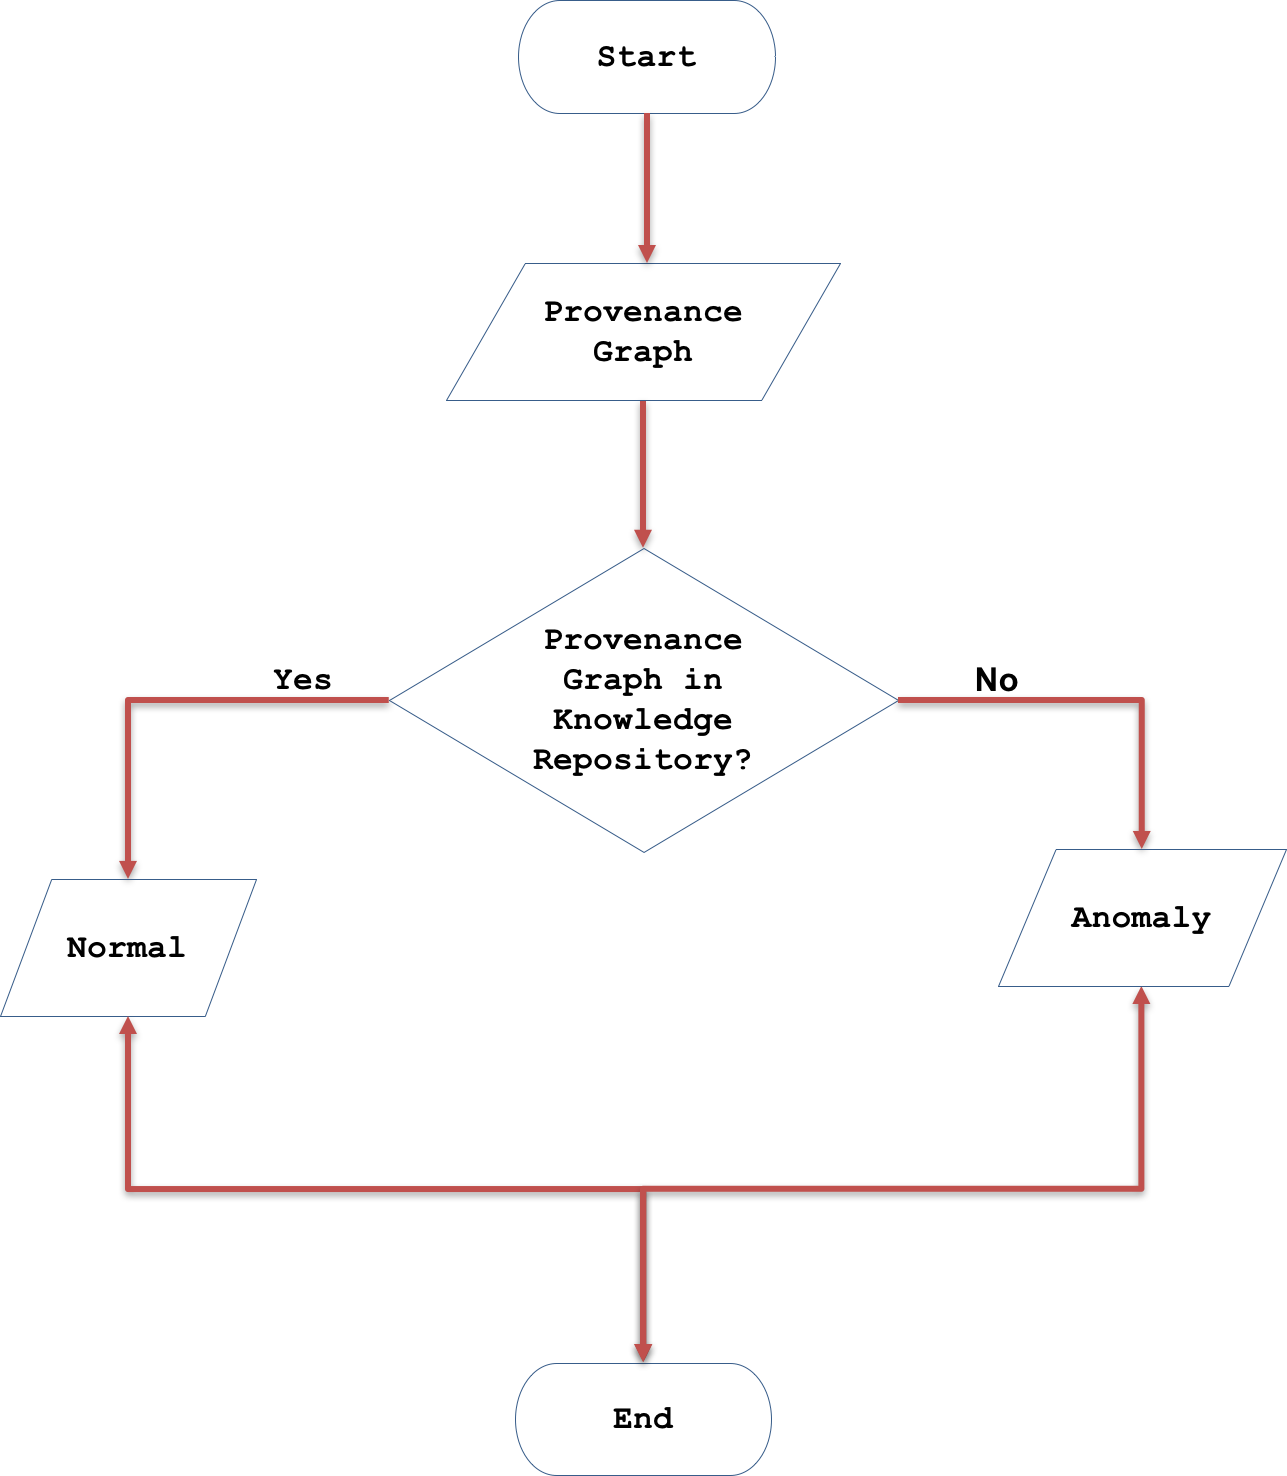
\includegraphics[height=4in, width=3.5in]{whitelist.png}
%\end{center}
%\caption{Whitelist approach to anomaly detection}
%\label{whitelist}
%\end{figure}


\subsection{Anomaly Detection on Provenance Graphs}

%The notion of what constitutes an anomaly is often domain specific. Hawkins defines an anomaly as an ``observation which deviates so much from other observations as to arouse suspicion that it was generated by a different mechanism" \cite{hawkins}. In computing, an anomaly often indicates the presence of a malicious intrusion or a system fault. For example, an anomaly could be a sudden increase in web traffic on a web server which could be indicative of a denial of service attack. Additionally, in a critical care health device such as a pacemaker, an anomalous event could be detrimental to the health of a patient which could result in the loss of life. 

%Anomaly detection consists of two phase, learning phase also known as the training phase and the test also known as the detection phase. In the training phase, the system collects training dataset. This data is considered to be a representation of the system's normal daily activity and free from malicious events. Once training dataset has been collected, the system's activities are further observed. This part is known as the testing phase. In the testing phase,  observed system behavior is compared to the learning phase to determine is an anomaly exists between the two. A threshold as defined by domain experts is used to determine if the observed data is considered an anomaly.

%Data labels are grouped into three major categories. Supervised anomaly detection, semi-supervised anomaly detection, and unsupervised anomaly detection. In supervised anomaly detection approach, training data contains instances of normal and anomalous data. Incoming data is classified based on the training data category. In semi-supervised approach, only one class of training data is collected, normal data. Incoming data that does not fit the normal class as specified by a threshold is regarded as an anomalous. In the training phase, most anomaly detection techniques use data derived from the normal system behavior.  This is referred to as one class classification. In unsupervised approach, there are no training dataset. it is believed that normal data is clustered around each and occurs more frequently than an anomaly. This is a widely used form of anomaly detection since training data which is hard to get is not requited. 







%Graphs offers a means of modeling complex structures such as social networks, computer networks, biological DNA sequences.  




%Details on anomaly detection techniques are outlined below
%
%
%\begin{enumerate}[]
%
%
%\item Statistical-based approach: This approach involves the use of parametric or non parametric statistical inference to develop models which are used to determine if a dataset fits a statistical model. Instances that do not fit the defined statistical model are classified as an anomaly. 
%
%\item Classification: The main idea in this approach involves building models which use training data set with predefined labels (i.e normal, anomalous) to classify incoming data. Classification works in two phase: training phase and observation phase. In the training phase, data is collected which contains labels of normal and anomalous system behavior. If the dataset only contains a label of either anomalous or normal behavior, this is considered as a one class classifier. In the observation phase, incoming data is classified by defined data labels.
%\begin{itemize}
%
%\item Nearest-Neighbor: It is based on the assumption that normal data occurs in dense neighborhoods and abnormal data in sparse neighborhoods. The main idea is to assign an incoming observation data to a class based on its proximity to the closest data point in the training data set. A distance or similarity measure is used to quantify the distance between points in a dataset.  A popular form of nearest neighbor technique is the $k$-nearest neighbor which groups incoming data based on proximity to $k$ closest data point. Details on $k$- nearest neighbors is discussed in section 3.5. 
%
%\end{itemize}
%
%\item Clustering: The main idea is to group similar data instances into clusters. There are various approach to clustering. One approach looks at the density of the clusters, normal data belongs to large dense clusters while abnormal data belongs to small clusters. Another approach as treats clustering as one class which assumes that normal belongs to a cluster and abnormal data does not. Another approach looks at the distance of the data to the centroid. Centroids are seen as the center of the cluster. Normal data are  considered to be closer to the centroid than anomalies lie.
%
%\begin{itemize}
%
%\item Density: This approach is used to estimate the density of  $k$ nearest neighbors. A data instance in a dense neighborhood is considered normal while data instances in neighborhoods with a sparse density are considered anomalous. The distance from a data instance to a nearest neighbor is seen as the inverse of the density of data instances.  This approach faces an issue in which the density approach performs poorly in regions of varying densities. Local outlier factor addresses this issue. Local outlier factor is a measure of the degree of Outlieriness of each data instance contained in a data set. It is achieved by comparing the ratio of local density of k nearest neighbors to the density of a data instance. Data instances with lower density are considered outliers.
%
%\end{itemize}
%
%
%
%
%
%
%\end{enumerate}    

Anomaly detection involves the use of rule-based, statistical, clustering or classification techniques to determine normal or anomalous data instances. The process of determining all anomalous instances in a given dataset is a complex task. A major challenge in anomaly detection is providing the right feature set from the data to use for detection. Another challenge exists in defining what constitutes as normal system behavior. Most anomaly detection using point-based data often fail to include the dependencies that exist between data points. 

\par Due to the ubiquitous nature of IoT devices, there are a wide array of vulnerabilities associated with them. In designing our anomaly detection framework, we expect an attacker's footprint is reflected through the data flow as depicted in the provenance graph. Our algorithm detects attacks such as false data injection, and state change as depicted in information flow of sensor events in provenance graphs.

\par Many IoT devices implement a control systems in which sensor data is used as an input in a feedback loop to an actuator. The operations of most control systems are regular and predictable. For example, in a thermostat application, temperature readings generated might be converted from Celsius to Fahrenheit and utilized as feedback to an actuator. Each iteration of a control loop sequence generates a path in a provenance graph. This notion can be leveraged to define an expected provenance graph for each application. 
\par The expected regularity of provenance graphs in IoT applications motivates a supervised learning approach to anomaly detection. This approach consists of two phases: observation phase, also known as the training phase, and the detection or test phase. In the observation phase, the system collects provenance data considered to be a representation of the normal system behavior. In the detection phase, the provenance graph set is compared with the provenance graph derived from subsequent observations to determine if an anomaly exists by measuring similarity between this graph and the provenance graph set. \textcolor{red}{Note that provenance graphs from the observation and detection phase form a graph set. A global edge set, $E_G$ represents the union of edge sets contained in a graph set. Algorithm \ref{alg:graph_anomaly} is the graph anomaly detection function given an observation phase graph set, $P$, and a detection phase graph, $p$. $Z$ represents a list of the cosine scores from comparing each of the provenance graphs in the observation phase graph set with a detection phase graph. A  function, $calculateAnomalyScore$ is used to determine the anomaly score, which is based on the minimum cosine similarity score of elements contained in $Z$.}

%minimum cosine similarity score of each element contained in $Z$.}
%
%
% it calculated the anomaly score, which is currently based on the minimum cosine similarity in Z.

%Each provenance graph contained in the detection phase is compared to provenance graphs contained in the observation phase with the result being a list of cosine similarity scores $Z$.

%We call the graphs collected from the observation and detection phase the provenance graph set.


%\section{Graph Similarity Anomaly Detection}



%Given $u_x, u_y$, the vector representation of provenance graphs $p_x, p_y$. Similarity of $p_x, p_y$ is found by calculating the cosine similarity between t$u_x$ and $u_y$. A threshold value is used to classify the behavior of provenance graphs in the detection phase as normal or an anomaly.


%since all generated vectors are derived from its ordering.


% \par Selecting the most appropriate feature from provenance graphs is an important task. We need to utilize features that preserve the order of edges and nodes contained in the provenance graph. Our approach utilizes the occurrence of unique edges contained in both graphs.  


%\par To determine identical edges, we utilize a combination of edge labels and source and destination node. That is, for two edges to be considered identical, they must contain identical labels and contain identical source and destination nodes. We say two edges $E_x $ and $E_y$ are identical (denoted $E_x \sim E_y$) if $E_x.V_s = E_y.V_s$, $E_x.V_d = E_y.V_d$, and $E_x.label = E_y.label$.  



%\begin{figure}[h!]
%\begin{center}
%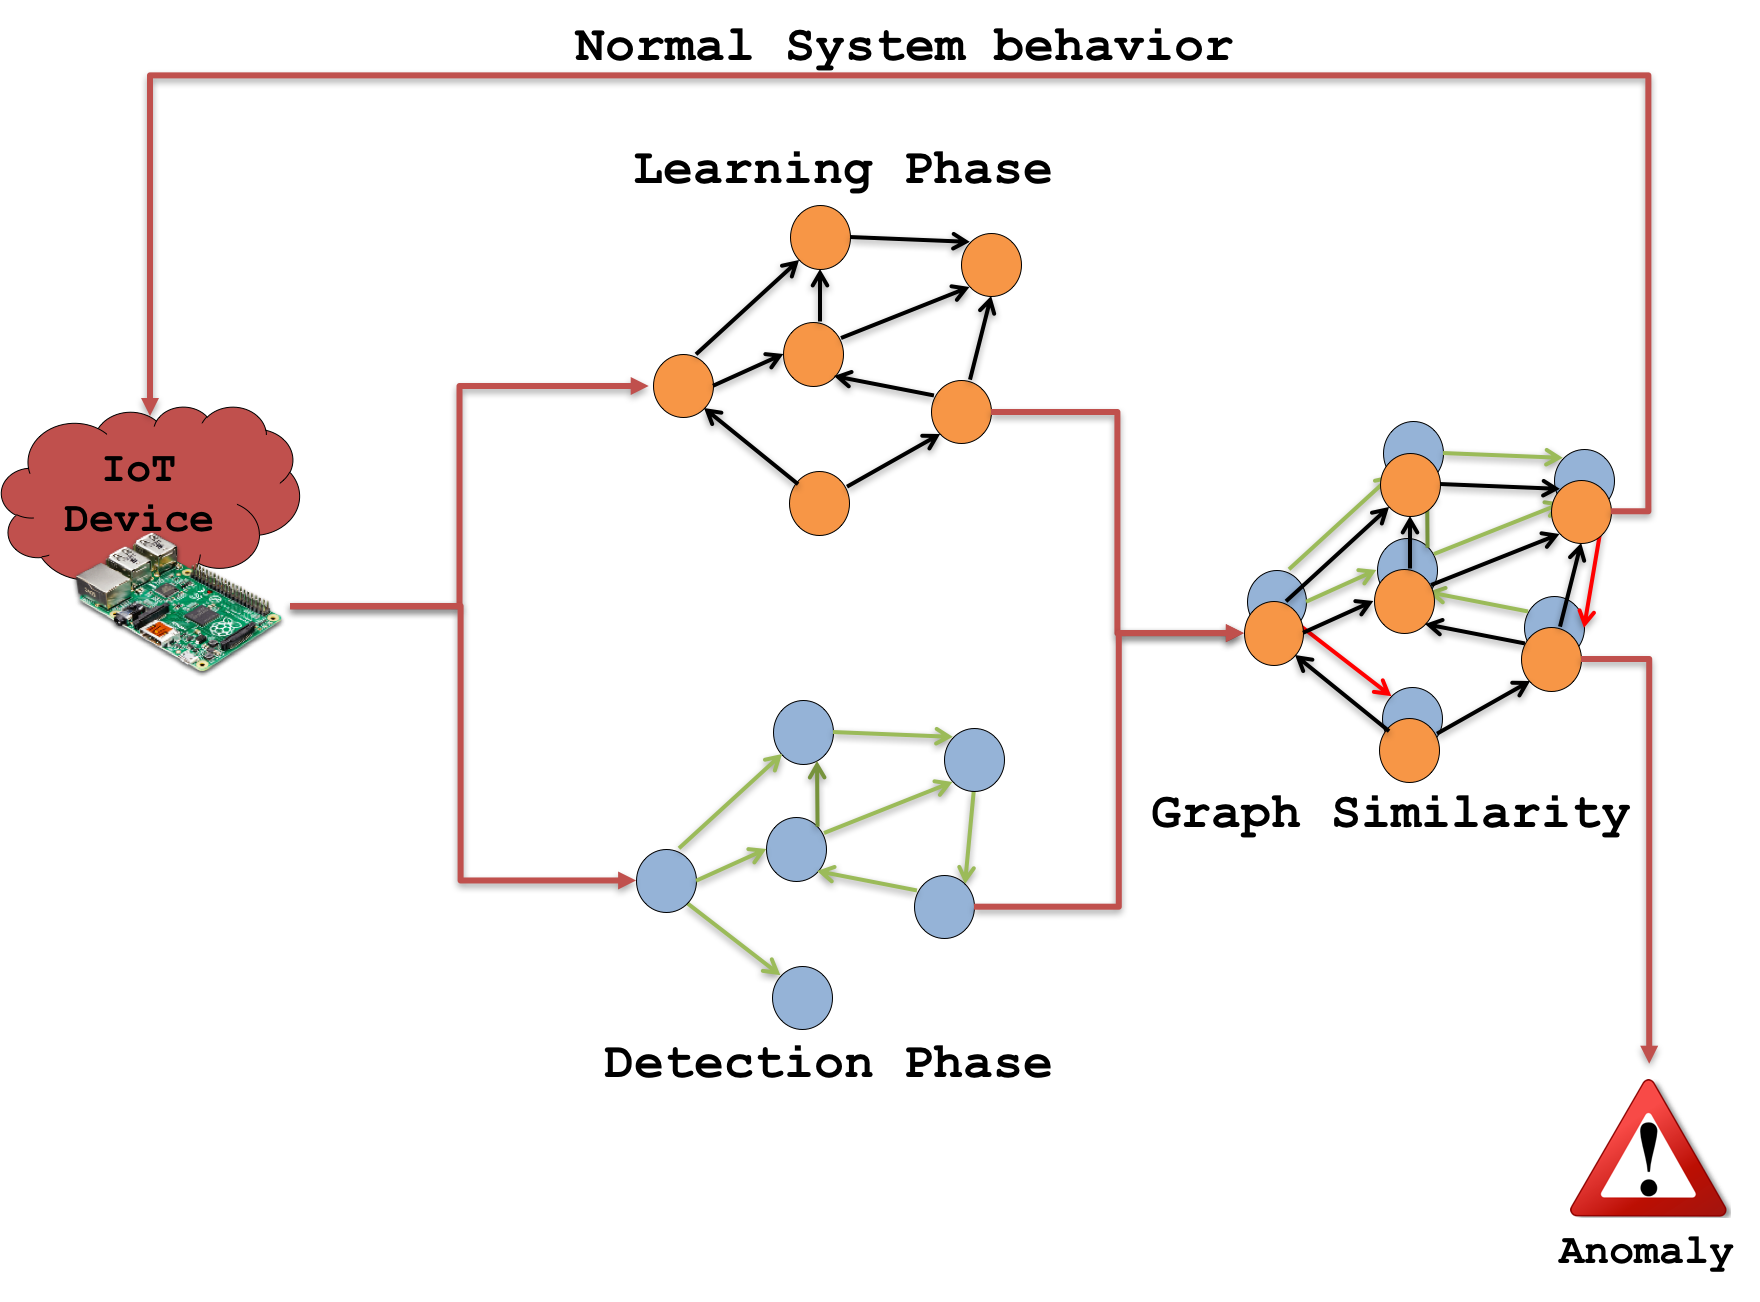
\includegraphics[height=2.5in, width=3.5in]{similarity_5.png}
%\end{center}
%\caption{Graph Similarity Approach}
%\label{graph_similarity}
%\end{figure}

%\par In performing our graph to vector space conversion, we define a set of procedures. First, we define our edge identification function as follows: 


%\begin{definition}
%
%%Consider a provenance graph, $p = (V, E)$ where $E = \{E_i,...E_n\}$ and $E_i = (n_s, n_d, label)$. $n_s, n_d$ are source and destination vertices respectively $ \mid n_s, n_d \in V$.  The equivalency function of two edges $eq(E_x, E_y)$  is $ E_x = E_y  if E_x \rightarrow n_s  \&  E_y \rightarrow n_s $  
%
%%Consider a provenance graph, $p = (V, E)$ where $E = \{E_0,...E_n\}$ and $E_i = (n_s, n_d, label)$. $n_s, n_d$ are source and destination nodes respectively such that $ n_s, n_d \in V$. Edges $E_x $ and $E_y$ are considered identical if $E_x.n_s = E_y.n_s$ and $E_x.label = E_y.label$  
%
%
%Consider a provenance graph, $p = (V, E)$ where $E = \{E_1,...E_n\}$ and $E_i = (V_s, V_d, label)$. $V_s, V_d$ are source and destination vertices respectively such that $ V_s, V_d \in V$. The edge identification function $\delta$ is defined as:  $E_x $ and $E_y$ are considered identical (i.e. $E_x \sim E_y$) iff $E_x.V_s = E_y.V_s$, $E_x.V_d = E_y.V_d$, and $E_x.label = E_y.label$  
%
%\end{definition}
 





%Edges contained in a provenance graph yet distinct could posses identical edge labels that can be utilized. 





%\begin{figure}[h]
%\begin{center}
%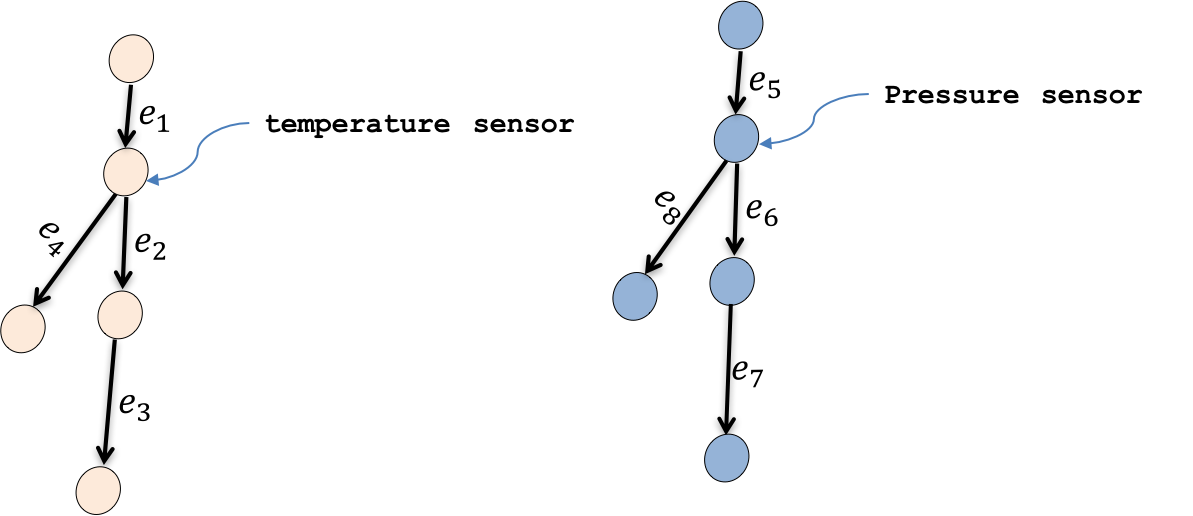
\includegraphics[height=1.7in, width=3.5in]{sensor_vector.png}
%\end{center}
%\caption{Edge identification between two graphs. Identical events from Different sensor nodes corresponds to different edges}
%\label{example}
%\end{figure}





%\begin{definition}
%
%%Let $P = \{p_1,...,p_n\}$ such that $p_i = (V, E)$. $E_{G} = \{ e_1,...,e_n\} \mid E_{G}  \in P$ where $e_i \neq e_{i+1}, 1 \leq i \leq n$. $E_{p} \gets \{e_1,...,e_n\} \mid E_{p} \in p$ where  $e_{pi} \neq e_{pi+1}, 1 \leq i \leq n$
%%
%\end{definition}
%
%
%Finally, we define our provenance graph to vector approach as follows:

%\begin{definition}
%Let $P = \{p_1,...,p_n\}$ where $p_i = (V, E)$. The vector space representation of $p_i, \boldsymbol{u_i}$, is the number of times edges contained in $E_G$ occurs in $E_p$. $\boldsymbol{u_i}$ has a length of $n$ which consists of all of the unique edges contained in the global edge list $E_G$
%
%\end{definition}





%Unique edges are found by identifying similar edges and a frequency count of the number of edges. 


 
%
%\[ \boldsymbol{v_x} = ( freq(E_i, p_i)) \]
%
%where $freq$ denotes the occurrence of $E_i$ in graph $p_i$







%\[ \boldsymbol{v_1} = (2,1,1,1,1) \] \[\boldsymbol{v_2} = (1,2,0,1,1,1,0) \]

%\begin{figure}[h]
%\begin{center}
%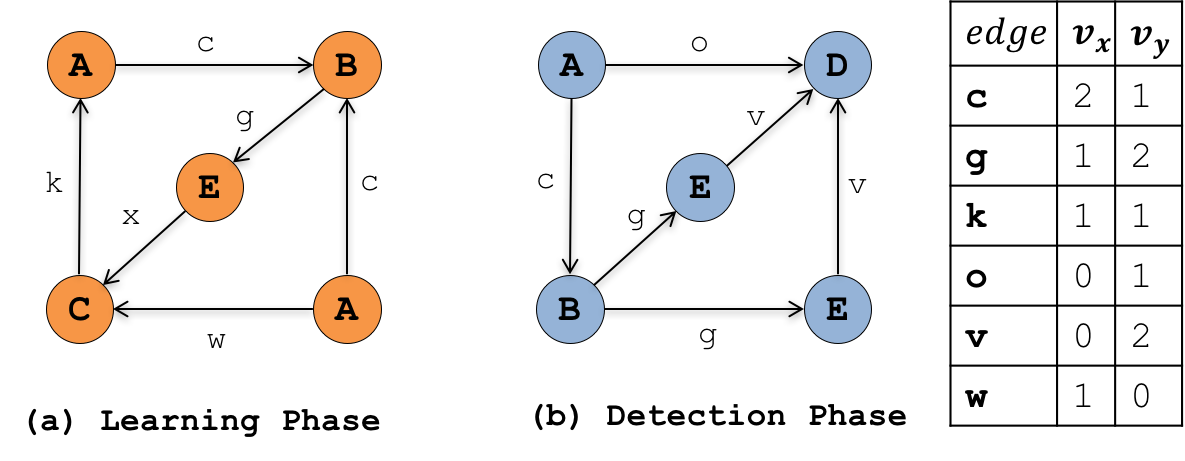
\includegraphics[height=1.7in, width=3.5in]{graph_sim_update.png}
%\end{center}
%\caption{Provenance graphs and their vector representation. $v_x, v_y$ represents the vectors generated from the learning and detection phase respectively}
%\label{example}
%\end{figure}



%\begin{multicols}{2}
%\lipsum[1-7]
%\end{multicols}




%\subsection{Graph Based Similarity Detection Algorithm}



%\[sim(u_x,u_y) =  \dfrac{u_x \cdot  u_y}{ \lVert \mathbf{u_x} \rVert \cdot \lVert \mathbf{u_y} \rVert} =\dfrac{\sum_{i=1}^n u_{xi} u_{yi} }{\sqrt[]{\sum_{i=1}^n u_{xi}^2} \times \sqrt[]{\sum_{i=1}^n u_{yi}^2}}  \in [0,1] \]

\begin{algorithm}
\caption{Cosine similarity given two vectors.}
 \label{alg:graph_similarity}
 
\begin{algorithmic}[1]

\Procedure{sim}{$u_x,u_y$}
\State \textbf{INPUT: } $u_x=\{u_{x_0},...,u_{x_n}\},u_y=\{u_{y_0},...,u_{y_n}\}$
\State $S_p, S_{u_x}, S_{u_y} \gets$ 0
%\State $S_{ux} \gets$ 0
%\State $S_{uy} \gets$ 0
\For{$ 0 \leq i \leq n$}

\State $S_p \gets S_p + (u_x[i] \times u_y[i])$
\State $ S_{u_x} \gets  S_{u_x} + u_x[i]^2$
\State $S_{u_y} \gets S_{u_y} + u_y[i]^2$

\EndFor

\State $G \gets \dfrac{S_p}{\sqrt[]{S_{u_x}} \times \sqrt[]{S_{u_y}} }$

%\State $G \gets S_p \div \sqrt[]{S_{ux} \times S_{uy}}$

\State \textbf{return} $G$

\EndProcedure

\end{algorithmic}

\end{algorithm}

\begin{algorithm}
\caption{Algorithm to construct the global edge set}

\begin{algorithmic}[1]  
\caption{Construction of global edge set from a set of provenance graphs.}
\label{graph_to_globaledgelist}

\Procedure{GraphSetToGlobalEdgeSet}{$P$}
\State \textbf{INPUT: } $P=\{p_0,...,p_n\} \mid p_i\gets (V_i, E_i), 0 \leq i \leq n.$

%\State $E_G \gets \{\}$
%\For{$p_i = (V_i, E_i) \in P, 0 \leq i \leq n$}
\State \textcolor{red}{$E_G \gets \cup_{i=0}^{n} E_i$}

%\EndFor
\State \textbf{return} $E_G$

\EndProcedure

\end{algorithmic}
\end{algorithm}


%%% copied algorithm

%\begin{algorithm}
%\caption{Algorithm to construct the global edge list}
%
%\begin{algorithmic}[1]  
%\caption{Global edge list algorithm given a set of provenance graphs, $P$.}
%\label{graph_to_globaledgelist}
%
%\Procedure{GraphSetToGlobalEdgeList}{$P$}
%\State \textbf{INPUT: } $P=\{p_0,...,p_n\} \mid p_i\gets (V_i, E_i), 0 \leq i \leq n.$
%
%\State $E_G \gets \{\}$
%\For{$p_i = (V_i, E_i) \in P, 0 \leq i \leq n$}
%\For{$e_j \in E_i$}
%\State \textit{Found} $\gets$ False
%\For{$e_g \in E_G$}
%\If{$e_j \sim e_g$}
%\State \textit{Found} $\gets$ True
%\EndIf
%\EndFor
%\If{\textit{Found} = False}
%\State $E_G \gets E_G \cup e_j$
%\EndIf
%
%\EndFor
%
%\EndFor
%\State \textbf{return} $E_G$
%
%\EndProcedure
%
%\end{algorithmic}
%\end{algorithm}


\begin{algorithm}[h!]  
\caption{Graph to vector conversion.} 
 \label{graph_to_vector} 
\begin{algorithmic}[1]

\Procedure{GraphtoVector}{$E, E_G$}

\State $n \gets |E_G|$

\State $Q[k],Q[i] \gets 0, 0 \leq i < n$

\For{$e_j \in E$}

%\State \textit{Found} $\gets$ \textbf{False}

\For{$e_g \in E_G \mid 0 \leq g < n$}

%\If{$e_j \sim e_g$}
\If{$e_j = e_g$}
\State $Q[g] \gets Q[g] + 1$
%\State \textit{Found} $\gets$ \textbf{True}
\EndIf

\EndFor

\EndFor


\State \textbf{return} $Q$

\EndProcedure

\end{algorithmic}
\end{algorithm}

\begin{algorithm}[h!] 
\caption{Calculates an anomaly score given a set of cosine similarity values.}  
 \label{alg:min_func} 
\begin{algorithmic}[1]  

\Procedure{calculateAnomalyScore}{$Z$}
\State \textbf{INPUT: } $Z=\{z_0,...,z_n\} , 0 \leq i \leq n.$
\State score $\gets 0.0$
\For{$z_i \in Z$}
\If{score $> z_i$}
\State score $\gets z_i$
\EndIf
\EndFor	
\State \textbf{return} score
\EndProcedure

\end{algorithmic}
\end{algorithm}


\begin{algorithm}[h!]

\caption{Detection algorithm given an observation phase graph set, $P$, a detection phase graph, $p$, and a $threshold$.} 
 \label{alg:graph_anomaly} 

\begin{algorithmic}[1]  

\Procedure{GraphAnomaly}{$P,p,threshold$}

\State $E_G \gets GraphSetToGlobalEdgeSet(P \cup p)$

\State $Q \gets GraphtoVector(p, E_G)$ 

\State $Z \gets \{\}$

\For{$p_i \in P$}
\State $N_i \gets GraphtoVector(p_i, E_G)$

\State $z \gets SIM(Q, N_i)$

\State $Z \gets Z \cup z_i$

\EndFor	

\State $s_{val} \gets calculateAnomalyScore(Z)$

\If{ $s_{val} \geq$ threshold}
\State \textbf{return} normal

\EndIf

\State \textbf{return} anomaly
\EndProcedure



\end{algorithmic}



\end{algorithm}



%\begin{figure}[h!] \label{alg:graph_anomaly} 
%
%\begin{algorithmic}[1]  
%
%\Procedure{GraphAnomaly}{$P,p$}
%
%\State $E_G \gets GraphSetToGlobalEdgeList(P \cup p)$
%
%\State $Q \gets GraphtoVector(p, E_G)$ 
%
%\For{$p_i \in P$}
%\State $N_i \gets GraphtoVector(p_i, E_G)$
%
%\State $z \gets SIM(Q, N_i)$
%\If{z $\geq$ threshold}
%\State \textbf{return} normal
%
%\EndIf
%
%\EndFor	
%
%\State \textbf{return} anomaly
%\EndProcedure
%
%\caption{Graph based anomaly detection algorithm} 
%
%\end{algorithmic}
%
%
%
%\end{figure}


%\subsubsection{Algorithm}




%\subsubsection{Defining Anomaly Threshold}
%
%An anomaly threshold $t$ is a score that defines at what point a provenance graph contained in the test data is considered anomalous. Ensuring a proper threshold score is used for detection is an important task that requires extensive knowledge of the application domain. The threshold is manually set to a value $t$, which is defined by domain experts. For automatic anomaly threshold detection, one can use prediction methods to define an anomaly score. Prediction techniques are beyond the scope of this paper. 

%\subsubsection{Computational Complexity:}
%
%\textcolor{red}{  TODO}

%\subsection{Threat Model and Assumptions}
%Due to the ubiquitous nature of IoT devices, there are a wide array of vulnerabilities associated with them. In designing our anomaly detection framework, we expect an attacker's footprint is reflected through the data flow as depicted in the provenance graph. Our algorithm detects attacks such as false data injection, and state change as depicted in information flow of sensor events in provenance graphs.


\section{Experiment}

The experiment evaluation serves as a preliminary study to confirm the correctness of our theoretical approach in detecting anomalous instances between provenance graphs. We evaluate our intrusion detection algorithm by implementing an IoT application which simulates a climate control system. Climate control systems ensure a proper functional environment for people and machinery. Constant irregularities in temperature could have devastating effects on industrial machinery. This system consists primarily of a heating ventilation and air conditioning (HVAC) system which uses temperature and humidity data to regulate environmental conditions within a building. We utilize a publicly available dataset \cite{LANGEVIN201594} which consists of a year's worth of longitudinal data on the thermal conditions, related behaviors, and comfort of twenty-four occupants in a medium-sized building generated at  a period of fifteen minutes. We utilize the temperature and humidity data as input to our simulation. We generate provenance graphs for each week of the year. We compare the provenance graph generated in consecutive weeks to see how they differ using our graph similarity approach (i.e., week 1 compared to week 2, week 2 compared to week 3 etc.). 
\par Figure \ref{figure} depicts the cosine similarity between provenance graphs generated from the first occupant by preceding weeks.  \textcolor{red}{ Since the dataset does not contain attacks, these rapid decline would likely indicate false positives. This might also be as a result of rapid variation in temperature change for each week in the given dataset.}

%The rapid decline in the graph is as a result of anomalies between the provenance graphs. This might be as a result of rapid variation in temperature change for each week in the given dataset.  

\textcolor{red}{ Ensuring a proper threshold score is used for detection is an important task that requires extensive knowledge of the application domain. The threshold is manually set to a value which is defined by domain experts. For automatic anomaly threshold detection, one can use prediction methods to define an anomaly score. As an example, a threshold might be set to $0.15$ in which all of the scores below the threshold are considered anomalous.}

\begin{figure}[tb]
\begin{center}
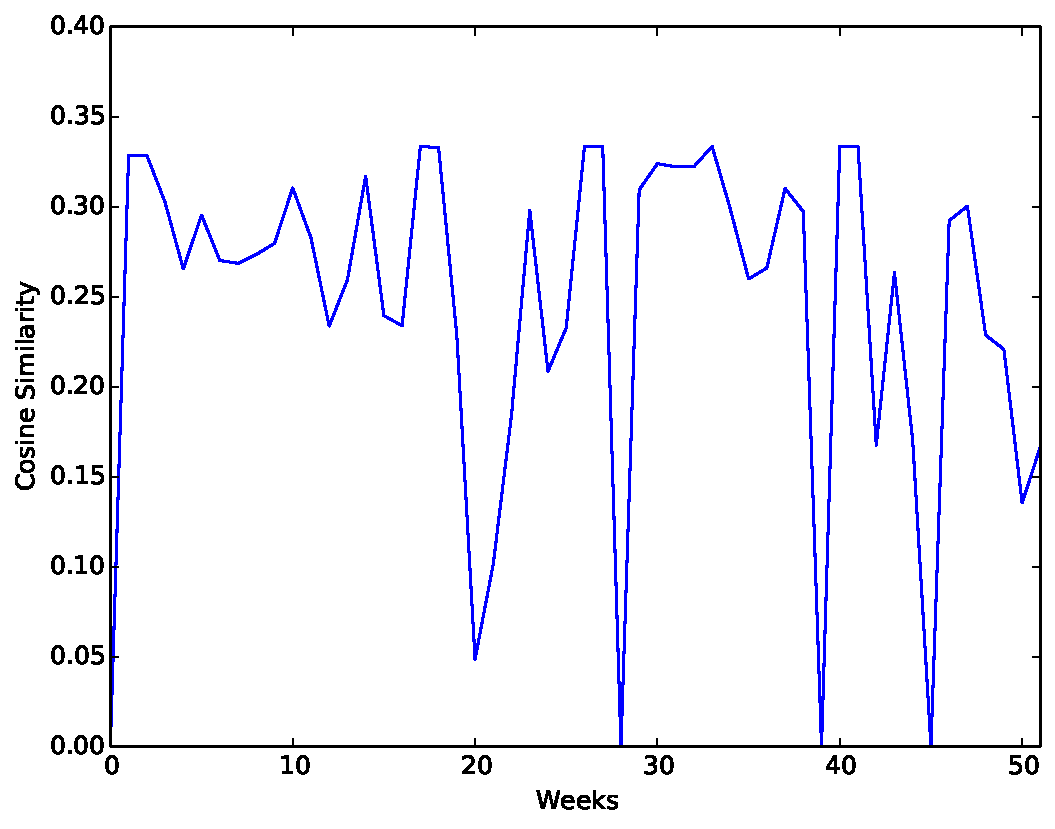
\includegraphics[width=\columnwidth]{foo.pdf}
\end{center}
\caption{Provenance graph comparison of climate control system by week.}
\label{figure}
\end{figure}



%We evaluate the performance of our proposed algorithms by calculating three performance metrics: false positive, true positive and false negative rate. False positive indicates when an intrusion that does not exist is detected, false negative indicates when the IDS classifies a provenance graph as normal when it is malicious, finally for true positive an IDS classifies a provenance graph as anomalous which is actually an intrusion.  Detection rate, false alarm rate and false negative rate are calculated as follows: 
%
%  \[Detection\, rate =  \dfrac{TP }{TP + FN}\] 
%  \[False\, alarm\, rate =   \dfrac{FP }{FP + TN}\] 
%  \[False\, negative\, rate =  \dfrac{FN }{FN + TP} \]


%Provenance graphs were generated using an IoT applications running on the raspberry pi 3. The first application simulates a Heating Ventilation, AC system and the other application simulates a. To generate malicious attack dataset, we utilized simulated data of how provenance graphs will look in an event of an attack. This graph was generated and agreed on by domain experts. To build our knowledge repository, we ran our IoT applications and the resultant provenance graph is stored in Neo4j, a graph database for efficient graph processing.


%\subsection{Discussion}
%
%\textcolor{red}{TODO}

%\section{Discussion and Limitations}
%\textcolor{red}{For experimentation, we only compare two graphs instead of a graphset. Online anomaly detection. Our anomaly detection system works best for offline intrusion detection.
%Static source code instrumentation. Offline anomaly detection tecnique. Future work would include real-time detection.
%
%
%}


\section{Related Work}

There has been a considerable amount of research done on contextualized event-based anomaly detection of system call sequence. Liao et al \cite{liao_using_2002} characterizes a system's normal behavior by denoting the frequency of unique system calls which are converted into a vector space representation. A classification algorithm such as $k$-Nearest Neighbors was used to classify the training data set. Stephanie et al. \cite{Hofmeyr} defines a human immune system inspired intrusion detection systems analyzing system call sequences of an application. Yoon et al. \cite{Yoon} developed a technique for intrusion detection on embedded systems by analyzing system call frequencies clustered using k-means which groups legitimate system behavior. Observations at run-time that do  not fit into a cluster are considered an anomaly. 
\par Additionally, anomaly detection on graphs has also been explored. Manzoor et al. \cite{manzoor_fast_2016} proposed a centroid based clustering anomaly detection for instances of streaming heterogeneous graphs in real time. Papadimitriou et al \cite{Papadimitriou2010} proposed five similarity algorithms for comparing the similarity of web graphs. Xie et al. \cite{Xie:2016:UID:2936026.2936232} proposed a provenance-aware intrusion detection and analysis (PIDAS) system using provenance graphs generated from system calls which reveals various interactions between files and processes. 
%PIDAS consists of three phases: the collection phase in which the provenance of normal system activity is stored in a key-value store database, the detection phase which compares the provenance graph of an executing program with provenance graphs contained in the normal database using a path match algorithm. This algorithm generates a score which is used to determine if a graph is anomalous or benign and the analyzer phase which allows for search of provenance data to determine the point of intrusion. 
\par Our approach differs from prior work because we focus on anomaly detection through information flow sequence of sensor data as represented by provenance graphs. 


%\cite{Noble} proposed two algorithms for anomaly detection in graphs The first approach, looks at unusual substructures in graphs. This is achieved by inverting the subdue score of patterns that occurs frequently in a graph. Subdue is a method for detecting substructures within graphs. The values that produce high scores are flagged as anomalies. The second approach examines unusual subgraphs contained in a graph by iteratively using subdue algorithm to compress the graph. The idea behind this method is that subgraphs containing many common substructures are considered less anomalous than one with less substructures. 


%Some graph approach involve the use of a community-based approach in which dense regions of connected nodes are considered normal and nodes with high sparse regions which do not belong to any community are considered anomalous. \textit{AUTOPART} \cite{chakrabarti2004autopart} consist of nodes with similar neighbors are clustered together and the edges which do not belong to any cluster are considered as an anomaly. To detect communities, it achieves this task by reorganizing the rows and the columns of the adjacency list.

% Our approach of graphs similarity is similar to graph kernels and graph edit distance. graph kernels involves measuring the similarity between two graphs, graph edit distance looks at the number of operations required for a graph $G_1$ to be identical to $G_2$. 


\section{Summary and Conclusion}

In this paper, we propose an anomaly detection algorithm for detecting anomalous instances of sensor based events in an IoT device using provenance graphs. We evaluate our approach with a preliminary study on an IoT application which simulates a climate control system.  \textcolor{red}{Current implementation of our anomaly detection algorithm works with offline data. Future work would include implementation for real-time detection. } We also plan on conducting further experimentation to identify the false and true positive rates of our algorithm using select IoT application dataset. 




\section{Acknowledgment}
This research has been supported in part by US National Science Foundation (CNS grant No. 1646317). Any opinions, findings and conclusions or recommendations expressed in this material are those of the author(s) and do not necessarily reflect the views of NSF.



